% \renewcommand{\sd}[1]{#1}
 \newcommand{\sdOct}[1]{#1}
\newcommand{\re}{\mathit{e}}

\section{ponts to make earlier}

\subsection{one}
In the introduction show a method where
\begin{lstlisting}
    void cautious(untrusted : Object, acc: Account){
    PRE acc.passwd PRT-FROM untrusted
    POST acc.passwd PRT-FROM untrusted
     ...
        ext-call does not pass acc.pwd
     ...
   }
\end{lstlisting}

Even external object creation may return an old, preexisting object.
Nevertheless, we are able to prove the above. Make a diagram that has an untrust', which has access to a.pwd. 


\subsection{two}
In our setting, we must deal with the possibility  that any untrusted object may point to any other untrusted object.
Therefore, any reference given to an untrusted object may end up, in principle,  eventually given to all of them.
Therefore if there was an untrusted object $u$ that had reference to $o$,  and we knew that $o$ was protected from $z$ now, we are not
allowed   to deduce that $o$ will still be protected in the "deep" future.
However, if we consider the "shallow" future, we can do better than that.

Namely, if  before an untrusted call with receiver and arguments $\overline z$ we know that $o$ is protected from $\overline z$, and if we know that the internal objects do not leak $o$ to the the external world, then we know that during execution of the untrusted call (and also all nested trusted or untrusted calls), $o$ will be protected (ie no locally accessible external object will obtain direct access), and that after the call, $o$ will still be protected from $\overline z$.

Going back to the discussion where $u$ has a direct (un-mitigated?) reference to $o$, if at the untrusted call with receiver and arguments $\overline z$, we know that $o$ is protected from $\overline z$, then this does not preclude that $u$ has unmitigated access to $\overline z$, but it does precludes that any of  $\overline z$ has unmitigated access to $u$ (because if had, then it would also have had unmitigated access to $o$ itself).

\subsection{three}
NOTE: JAMES asked Do we need to worry about well-fomedness? Eg what if we had an assertion $3 \wedge 5 \rightarrow 66$?

\subsection{four}
Say that protected-from is a heap property, whereas protected is a heap-frame property.

\section{\SpecLang specifications}
\label{s:semantics}

 
In this section we define {the}  \SpecLang specification language.  
We first define an underlying programming language, \LangOO (\S \ref{sub:Loo}).
We then define an assertion language, \AssertLang, which can talk about the
contents of the state, as well as about protection (\S \ref{sub:SpecO}).  Finally, we define the syntax and
semantics of  \SpecLang
specifications (\S \ref{s:holistic-guarantees}).

 


\section{\LangOO -- the underlying object oriented programming languages}

\subsection{\LangOO syntax and semantics}
\label{sub:Loo} 
 \LangOO  is a {small}, imperative, sequential, 
class based, typed, object-oriented language, whose
fields are private to the class where they are defined -- similar to the one in OOPSLA\footnote{any differences?}.
The complete definition of \LangOO i 
{can be found in the appendices  \cite{necessityFull}.}
 A \LangOO state $\sigma$ consists of a 
heap $\chi$, and a  {stack $\psi$ which is a sequence of frames}.
A frame, $\phi$, consists of
local variable map, and a continuation, \ie a sequence of statements to be executed.
%{We use  $| \sigma |$ to describe the numbers of frames in the stack of  $\sigma$, i.e. the number of nested, currently active method calls.}
 A statement may assign to variables, create new objects and push them to the heap, 
perform field reads and writes on objects,  or
 call methods on those objects. 

 
Modules are mappings from class names to class definitions. 
Execution 
takes place
 in the context of  a module $M$ and   a state $\sigma$,
 defined via unsurprising small-step semantics of the form \ \ 
   $M, \sigma \leadsto \sigma'$.
The   top frame's continuation contains the statement to be 
executed next.  

\paragraph{Notation} We adopt notation from OOPSLA, where
 $\interpret{\phi}{x}$  indicates the value of $x$   in the local variable map of frame $\phi$, 
 and where $\interpret{\sigma}{x} = v$ means that $x$ 
maps to $v$ in the top-most frame of $\sigma$'s stack, and $\interpret{\sigma}{x.f} = v$
has the obvious meaning. The terms $\sigma.\prg{stack}$,  
$\sigma.\prg{contn}$,  
$\sigma.\prg{heap}$     mean the stack, 
the continuation at the
top frame of $\sigma$, %resp. 
and the heap of $\sigma$.
The term $\alpha\!\in\!\sigma.\prg{heap}$ means that $\alpha$ is in the domain of the heap of $\sigma$, and \emph{$x$ fresh in $\sigma$} means that 
$x$ isn't in the variable map of the top frame of $\sigma$, 
while the substitution  $\sigma[x \mapsto \alpha]$ is applied to the top frame of $\sigma$.
 \ $C\in M$ means that class $C$ is in the domain of module $M$. 


\paragraph{Applicability} 
{While our work is based on 
  a simple, imperative, typed, object oriented}
language with unforgeable addresses and private fields, we believe
 that % our approach
 it is applicable to several programming paradigms, and 
 that   unforgeability and privacy
 can be replaced 
 by lower level mechanisms such as capability machines \cite{vanproving,davis2019cheriabi}.

  \subsection{{Reachable  Objects}}
  
\sdOct{The  \SpecLang  specifications support universal quantification over  objects; such specifications 
are applicable  to all objects in the heap witch, are however, either locally reachable (i.e. there is in the heap a path from the an 
object on the top frame to the particular object), or globally reachable (i.e. there is in the heap a path from the an 
object on some frame to the particular object.)
In this section  we will formally define these concepts.}\footnote{TODO we need a better motivation for these concepts.}
 



We define  % $\Relevant \alpha \phi \sigma $ as the objects $\alpha$ which are reachable from   the fame $\phi$,
locally reachable, $ \LRelevant \alpha \sigma $, as  the objects  $\alpha$ which are reachable the top frame on the stack of $\sigma$,
and globally reachable, $\GRelevant \alpha \sigma$, as the objects  $\alpha$ which  are reachable from any  frame on the stack of $\sigma$.
 
\begin{definition} We define 
\begin{itemize}
\item
$ \LRelevant \alpha \sigma $ \ \ iff\ \  
$\exists \phi.[\ \sigma=(\phi\cdot\_, \_)$ and $\Relevant \alpha \phi \sigma\ ]$. % for some $\phi$
\item
$\GRelevant \alpha \sigma$  \ \ iff\ \  
$\exists \phi.[\ \sigma=(\_\cdot\phi\cdot\_, \_)$ and $\Relevant \alpha \phi \sigma\ ]$. % for some $\phi$
\end{itemize}
where\\
$\strut\ \ \ \  \ \ \ \ \ \ \Relevant \alpha \phi \sigma $  \ \ \ \ \ \ \ iff\ \  
$\exists n\in \mathbb{N}.\exists \prg{f}_1,... \prg{f}_n.\exists \prg{x}.[ \ \interpret{\sigma}{\phi(x).\prg{f}_1.....\prg{f}_n} = \alpha \ \ ]$.

\end{definition}


The lemma below says that 1) Any locally reachable object is globally reachable, and 
2) Any object which existed in the current  heap, and is globally reachable at some future point is globally reachable now: that is, 
no globally unreachable object may become reachable.\footnote{cite "only connectivity begets connectivity"}


\sdN{
\begin{lemma}
\label{lemma:relevant}
For all $\sigma$, $\sigma'$, for all objects $o$, and for all modules $M$:
\begin{enumerate}
\item
$ \LRelevant \alpha \sigma\ \ \Longrightarrow \ \   \GRelevant \alpha \sigma$
\item
$M, \sigma  \leadsto^*   {\sigma'} \ \wedge \  \GRelevant o {\sigma'} \ \wedge \ o\in dom(\sigma) \ \ \Longrightarrow \ \  \GRelevant o {\sigma}$
\item
\sdOct{TODO: finish\\
$\sigma'$ is $\sigma$ right after a method has been called  $\wedge \  \LRelevant o {\sigma'}  \ \ \Longrightarrow \ \  \LRelevant o {\sigma}$
}
\end{enumerate}
\end{lemma}
}
 
 \begin{figure}[htb]
\begin{tabular}{|c|c|c|}
\hline \\
\resizebox{3.5cm}{!}{
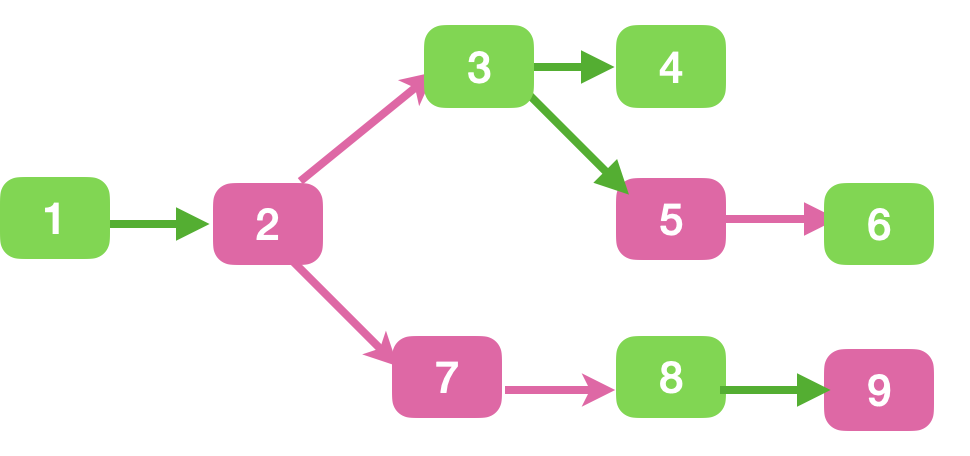
\includegraphics[width=\linewidth]{diagrams/heap.png}
} 
&
\resizebox{5cm}{!}{
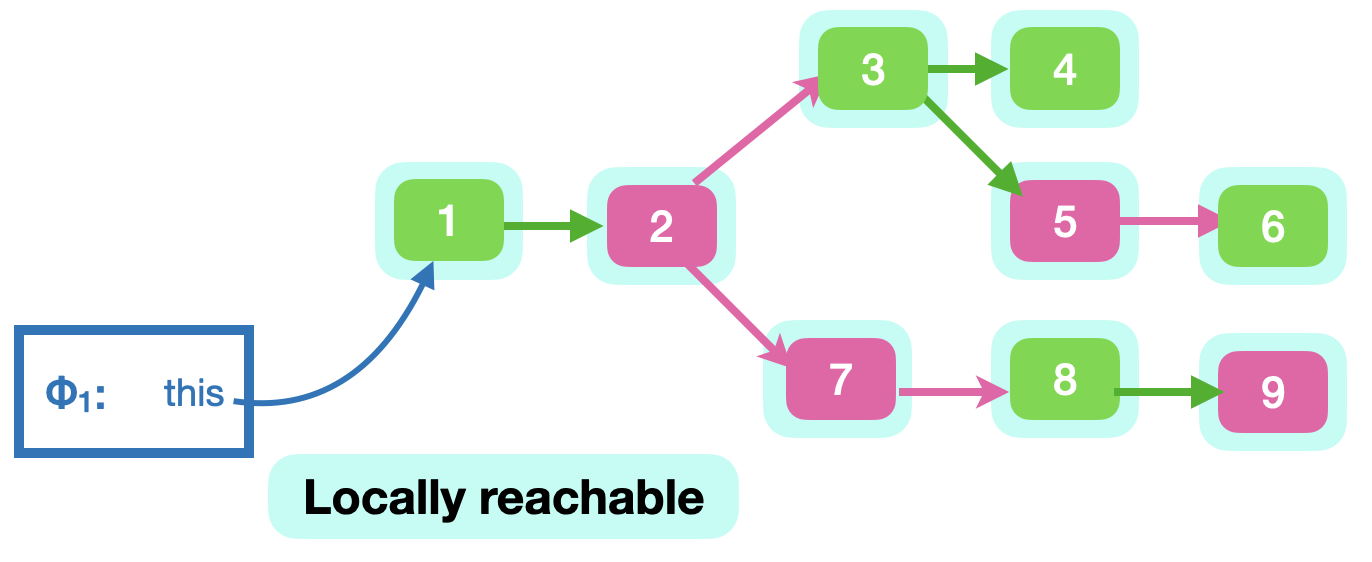
\includegraphics[width=\linewidth]{diagrams/locReachA.png}
} 
&
\resizebox{5cm}{!}{
\includegraphics[width=\linewidth]{diagrams//locReachb.png}
} 
\\
\hline
 a heap
&
Locally Reachable: ...
&
Locally Reachable \\
\hline \hline
\end{tabular}
   \caption{Locally Reachable Objects xxxx.  
 }
   \label{fig:LReachable}
 \end{figure}

  \subsection{Operational Semantics:  {deep} $\leadsto$ {and shallow} -- $\leadsto_{\sigma}$}\footnote{\sdOct{TODO: would be good to have a name for the latter: deep and shallow? or relative and absolute? something about horizons}}
\
\sdOct{In appendix ??? we give the operational small-steps semantics of \Loo; it has the shape $M, \sigma \leadsto \sigma'$. The semantics is un-surprising, except, perhaps for the fact that
it does not carry explicitly the instructions to be executed, as these are part of the frame. 
When a method is called, a new frame is pushed on to the stack of the state, and when we return from that call, its frame is  popped, and execution continues in the context of the calling method.
}
\begin{definition}[Deep semantics]
\label{def:deep}
We define the relation  $  {M} {\sigma_1} \leadsto  {\sigma_2}$ in appendix ...
\end{definition}

\sdOct{The $\leadsto-$semantics is deep, in that it allows  the current stack to grow and to also shrink. 
We illustrate this in the left side of  Fig. \ref{fig:UpSemantics}, where we depict a case where we are executing a method (say $m_a$), which eventually calls another method (say $m_b$), and which in tis turn calls a further method (say $m_c$): We start at $\sigma_1$ and in one step we reach $\sigma_2$, which is a method  call  to $m_b$. 
This leads to state $\sigma_3$, and after another step we reach $\sigma_5$, which is a method call to $m_c$, 
leading to state $\sigma_5$ and $\sigma_6$. 
The latter is the return, leading to $\sigma_7$, which again, is a return, leading to $\sigma_8$.}

\sdOct{For the purpose of $\SpecO$ specifications, where we require that some properties are invariant with time, we want the time/future to be shall, ie we do not want to ... \footnote{TODO write motivation} ...}

{
\begin{definition}[Shallow and terminating semantics]
\label{def:shallow:term}
We define the relation  $\leadstoRec {M} {\sigma_1} {\sigma} {\sigma_2}$\footnote{Could we give it a name? }
\begin{itemize}
\item
$\leadstoRec {M} {\sigma_1} {\sigma} {\sigma_2}$ \ \ \ iff \ \ \  ${M, \sigma_1} \leadsto {\sigma_2}$\\
$\strut  \hspace{3cm} \wedge $\\
$\strut  \hspace{2.7cm}\ \    \exists \phi,\psi, \phi_1, \phi2.[ \ \sigma = (\phi\cdot\psi,\_) \ \wedge \ \sigma_1 = (\psi_1\cdot \psi, \_)
\ \wedge\ \sigma_2 = (\psi_2\cdot \psi, \_)\ ] $ 
\item
$\Final {\sigma}$ \ \ \ iff \ \ \  $\exists \phi. [\ \sigma = (\phi\cdot\_,\_) \ \wedge \ \phi.\texttt{cont} \in \Values \ ]$
\item
$\leadstoFin {M} {\sigma} {\sigma'}$ \ \ \ P \ \ \  $\leadstoRecStar {M} {\sigma} {\sigma} {\sigma'} \ \wedge \ \ \Final{\sigma'}$.
\end{itemize}
\end{definition}
}

\footnote{TODO: use the diagram from Fig. 10 to explain deep and shallow execution}

\subsubsection{{Reachable  Objects and Shallow Semantics}}


The lemma below is the counterpart to lemma \ref{lemma:relevant}, but makes stronger assertions, because it only applies to shallow executions.\footnote{{It is more general than before!}}

\begin{lemma}
For all states $\sigma$, $\sigma'$, and $\sigma''$,for all objects $o$, and for all modules  $M$:
\begin{itemize}
\item
${\leadstoRecStar {M}  {\sigma} {\sigma''} {\sigma'}} \ \ \wedge \ \  \GRelevant o {\sigma'} \ \ \wedge\ \ o\in dom(\sigma)\ \ \ \Longrightarrow \ \  \ \GRelevant o {\sigma}$.
\item
${\leadstoRecStar {M}  {\sigma}  {\sigma''} {\sigma'}} \ \ \wedge \ \   \LRelevant o {\sigma'}\  \ \wedge\ \ o\in dom(\sigma)\ \ \ \Longrightarrow \ \ \ \LRelevant o {\sigma}$.
\end{itemize}
\end{lemma}



\section{\AssertLang -- the assertion language}
\label{sub:SpecO}

Our assertions language, \AssertLang, extends a 
 basic assertion language   with
object-capability assertions. 


\subsection{Syntax of \AssertLang}
The syntax of \AssertLang   is given in
Definition \ref{f:chainmail-syntax}.
An assertion may be an expression,   a query of the defining class of
  an object, the usual connectives and quantifiers, along 
with two non-standard assertion forms:
(1) \emph{Internal/external} and (2) \emph{Protection}, inspired by the capabilities literature, and
\footnote{{ TODO say how these relate with capability lit;  compare with 
 OOPSLA.}}


\begin{definition}
Assertions ($A$) in
\AssertLang are defined as follows:

\label{f:chainmail-syntax}
 \[
\begin{syntax}
\syntaxElement{A}{}
		{
		\syntaxline
				{{\re}}
				{{\re} : C}
				{\neg A}
				{A\ \wedge\ A}
				{A\ \vee\ A}
				{\all{x:C}{A}}
				{\ex{x:C}{A}}
		\endsyntaxline
		}
		{
		\syntaxline
				{\internal{{\re}}}
				{\external{{\re}}}
				{\protectedFrom{{\re}} {{\re}}} 
				 {\inside {{\re}}} 
		\endsyntaxline
		}
\endSyntaxElement\\
\end{syntax}
\]

\textbf{NOTE}  We allow addresses in assertions, and this allows   that we can write assertions like $\alpha.bal > 700$, but note that universal quantification over addresses  ($\forall \alpha:C.[A]$) is not supported -- but one can obtain that effects through $\forall x:C.[A]$


\footnote{{\textbf{NOTE} It also allows assertions like $a1.passwd \neq a2.passwd$, whereas in the past we would have written as
$\exists x,y.[\ a1.passwd=x \wedge  a2.passwd=y \wedge x\neq y\ ]$.}}


\end{definition}

\footnote{{TODO compare with oopsla }}



\subsection{Semantics of \AssertLang -- first part}
The semantics of \AssertLang   
is given in Definition \ref{def:chainmail-semantics}. 
Definitions (1)-(5) are standard.
 Note that Definitions (6)-(7) ...  TODO: explain!
% An illustration of the concept of reachable appears in the next subsection, in Fig. \ref{fig:Relevant}.

We   use the evaluation relation, $\eval{M}{\sigma}{e}{v}$,
which says that the expression $e$ evaluates
to value $v$ in the context of state $\sigma$ and module $M$.
As expressions in \LangOO may be recursively defined, their evaluation 
need not   % may not necessarily 
 terminate. Nevertheless, the logic of $A$ remains classical because recursion is restricted
to expressions, and not generally to assertions.
\footnote{We have taken this approach from \citeasnoun{FASE}, which also contains a mechanized Coq proof that assertions are classical \cite{coqFASE}.
%  The full
The semantics of $\hookrightarrow$ {is} unsurprising 
(see {the appendices %of the full paper 
\cite{necessityFull}).} } %Fig.\ref{f:evaluation}).



\begin{definition}[Satisfaction 
of Assertions by module and  state] 
\label{def:chainmail-semantics}
We define satisfaction of an assertion $A$ by a % program 
state $\sigma$ with 
 module $M$ as:
\begin{enumerate}
\item
\label{cExpr}
$\satisfiesA{M}{\sigma}{{\re}}$ \ \ \ iff \ \ \  $\eval{M}{\sigma}{{\re}}{\true}$
\item
\label{cClass}
$\satisfiesA{M}{\sigma}{{{\re}} : C}$ \ \ \ iff \ \ \  $\eval{M}{\sigma}{{\re}}{\alpha}\   \wedge \ \class{\alpha} {\sigma}= C$
\item
$\satisfiesA{M}{\sigma}{\neg A}$ \ \ \ iff \ \ \  ${M},{\sigma}\nvDash{A}$
\item
$\satisfiesA{M}{\sigma}{A_1\ \wedge\ A_2}$ \ \ \ iff \ \ \  $\satisfiesA{M}{\sigma}{A_1} \   \wedge \ \satisfiesA{M}{\sigma}{A_2}$
\item
$\satisfiesA{M}{\sigma}{A_1\ \vee\ A_2}$ \ \ \ iff \ \ \  $\satisfiesA{M}{\sigma}{A_1}\   \vee \ \satisfiesA{M}{\sigma}{A_2}$

\item
\label{quant1}
$\satisfiesA{M}{\sigma}{\all{x:C}{A}}$ \ \ \ iff \ \ \  
 {$\forall \alpha.[\ \GRelevant \alpha \sigma \wedge  \satisfiesA {M}{\sigma} {\alpha:C}  \ \Longrightarrow   \ \satisfiesA{M}{\sigma} {A[x/\alpha]}\ ]$.} 

\item
\label{quant2}
$\satisfiesA{M}{\sigma}{\ex{x:C}{A}}$ \ \ \ iff \ \ \  
 {$\exists \alpha.[\ \GRelevant \alpha \sigma \wedge  \satisfiesA {M}{\sigma} {\alpha:C}  \ \wedge \ \satisfiesA{M}{\sigma} {A[x/\alpha]}\ ]$.} 
\item
\label{cInternal}
$\satisfiesA{M}{\sigma}{\internal{{\re}}}$ \ \ \ iff \ \ \   $\satisfiesA{M}{\sigma}{{{\re}} : C} \ \wedge\ \ C \in M$
\item
\label{cExternal}
$\satisfiesA{M}{\sigma}{\external{{\re}}}$ \ \ \ iff \ \ \   $\satisfiesA{M}{\sigma}{{{\re}} : C} \ \wedge \ C \notin M$
\end{enumerate}
\end{definition}

\textbf{Notes:}  We use the $\Longrightarrow$ symbol in our meta-language to denote implication while $\rightarrow$ is part of Chainmail syntax.
\footnote{{TODO: explain that$x$ is fresh in $\sigma$  means that $x$ is not in the domain of the top frame, nor in the top continuation of $\sigma$.
 Note, the assumption $x$ is fresh in $\sigma$ has to be justified. Barendregt convention? Or say how we rename if $x$ is not free.}}
\footnote{{TODO: say that any assertion $A(e)$ can be understood as a shorthand for $\exists x. [ x=e \wedge A(x)]$. or  $forall x. [ x=e \rightarrow A(x)]$?? For example, the  assertion   ${\internal{e}}$ is a shorthand for $\exists x. [ x=e \wedge {\internal{x}}]$. QUESTION: do we need to talk about $=$ in the assertion language?}}
In most cases, satisfaction of an assertion not only depends on the state $\sigma$, but 
in some cases it also depends on the module: namely execution of expressions (\ref{cExpr}) might need to look up the definition of ghost fields  in $M$, while 
for internal or external provenance (\ref{cInternal} and \ref{cExternal}) we need to know all the classes defined in $M$.

TODO: Compare with Dafny (or others). Does univ. quantifier mean quantify over all allocated objects (Dafny), or over reachable objetcs?

\subsection{Semantics of Assertions - second part: Protection}\footnote{Can we think of a better name than protection?}

As we already discussed in the introduction\footnote{make sure we do discuss there}, in the object capabilities world permission (ie access to\footnote{cite MarkMiller thesis, and our Permission and Authority revisited} to a capability is a necessary precondition to some effect. In our work, we express this as lack of permission to the relevant capability implies that the given effect will never take place.
For this, we need the concept of "lack of permission".  

We define this lack of permission as "protected".  An object $o$ is protected from another, external, object $o'$, if $o'$ can obtain   $o$ only if 
some internal object is involved in giving access to $o$. In other words, $o$ cannot become reachable to $o'$ unless a method is executed on
some internal object. That is, $o$ is protected from $o'$ if any path from $o'$ to $o$ goes through at least one internal object.

\begin{definition}[Satisfaction 
of Assertions by module and  state -- continued; Protection] 
\label{def:chainmail-protectionFrom}
We continue the definitions in \ref{def:chainmail-semantics}, and define   
\begin{enumerate}
\item
\label{cProtected}
$\satisfiesA{M}{\sigma}{\protectedFrom{{\re}} {{\re_{o}}}}$  \ \ \ iff \\
  $\exists \alpha, \alpha_{o}. [\ $
\begin{enumerate}
\item $\eval{M}{\sigma}{{\re}}{\alpha} \ \ \ \wedge\ \ \  \eval{M}{\sigma}{{\re_{o}}}{\alpha_{o}},  \ \ \ \wedge\ \ \  \alpha \neq \alpha_{o}$\ \ \ \  and  
\item $\satisfiesA{M}{\sigma}{\external{\alpha_0}}$, \ \ \ \ \ \ and  
\item 
$\forall n\in\mathbb{N}. \forall f_1,...f_n.$\\
$
[\ \ \interpret{\sigma}{\alpha_{o}.f_1...f_n}=\alpha \ \ \  \Longrightarrow \ \ \ \exists k\!<\!n. \satisfiesA{M} {\sigma} {\internal{{\interpret{\sigma}{\alpha_{o}.f_1...f_k}}}} \ \ ]$
\end{enumerate}
\strut \hspace{.4cm} $]$
\end{enumerate}
\end{definition}

TODO: Justify the definitions and their subtleties. 

It follows directly from the Def. \ref{def:chainmail-protectionFrom} that any object is protected from any internal object --
this is expressed in the lemma below. Therefore, when we consider whether an object $o$ is protected from another object $o'$,  we only consider external objects $o'$.

\begin{lemma}
\label{lemma:internalProtects}
For all modules $M$, and states $\sigma$, and terms $\re$, $\re_0$:
\begin{itemize}
\item
$ \satisfiesA{M} {\sigma} {\internal{\re_o}}$\ \ \ \ implies \ \ \ \ \  $\satisfiesA{M}{\sigma}{\protectedFrom{{\re}} {{\re_{o}}}}$
\end{itemize}

\end{lemma}



JAMES' comment: If is possible that "we" do not know the complete heap (eg we only know about the green stuff.) how do we know whether an object is protected. The answer is that we do not know that it is protected, but we do know that our code guarnartees poreservation of proetcedness.
%Nevertheless, if the objecta are "riobust" then we can prove that some properties will be preserved. 

\footnote{
OLD COMMENTS: ${\inside {\_}}$  is central to thinking about capabilities. For example, the balance of an account whose
  password is  encapsulated/protected?  will not decrease in the next step.
  Often, API implementations contain objects whose capabilities, while  crucial for the implementation, if exposed,
would break the intended guarantees of the API. Such objects need to remain confined - see
such an example in Section \ref{s:examples}. 
}

\footnote{{\textbf{TODO} make the connection with domination}}

{\textbf{NOTE}  that the term $\re$ may mention ghost fields, but the paths $\alpha.f_1....f_n$ may not. We see that because the latter are interpreted in $\sigma$. That is, $\satisfiesA{M}{\sigma}{{\alpha_o.f_1...f_n}=\alpha}$ is weaker than $\interpret{\sigma}{\alpha_{o}.f_1...f_n}=\alpha$. TODO: write the latter as a lemma}


 


\begin{figure}[htb]
\begin{tabular}{|c|c|c|}
\hline \\
\resizebox{4.5cm}{!}{
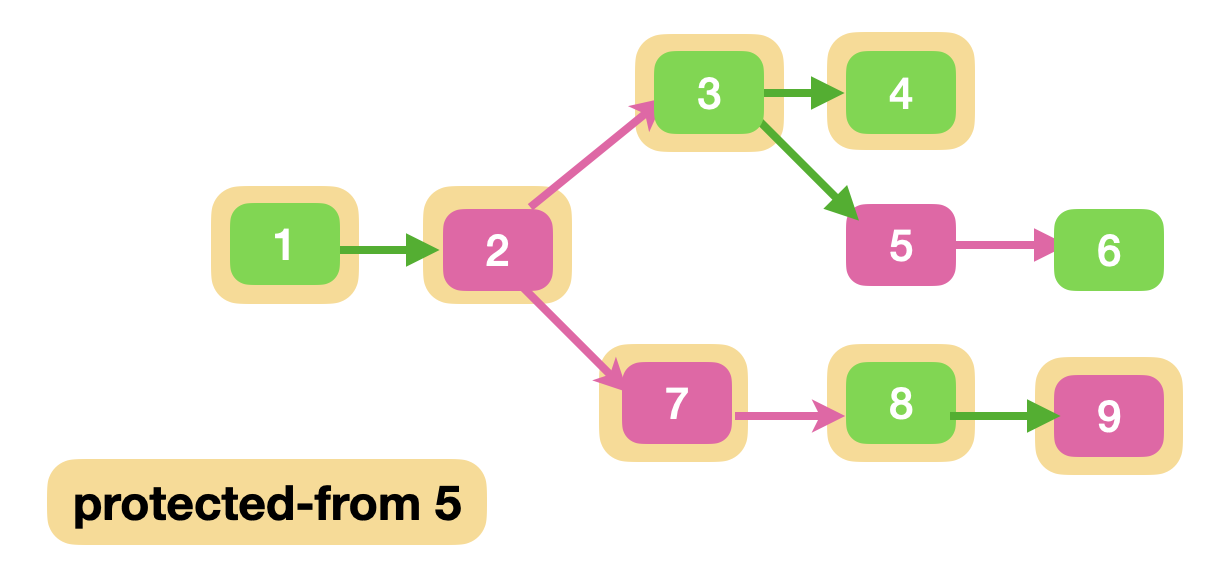
\includegraphics[width=\linewidth]{diagrams/prfA.png}
} 
&
\resizebox{4.5cm}{!}{
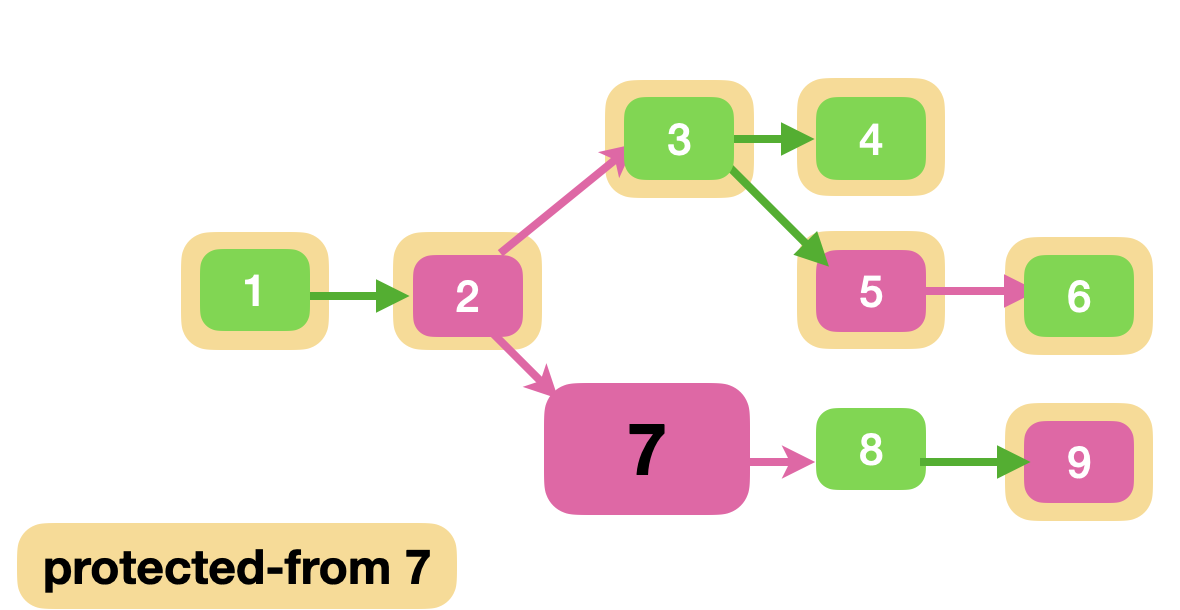
\includegraphics[width=\linewidth]{diagrams/prfB.png}
} 
&
\resizebox{4.5cm}{!}{
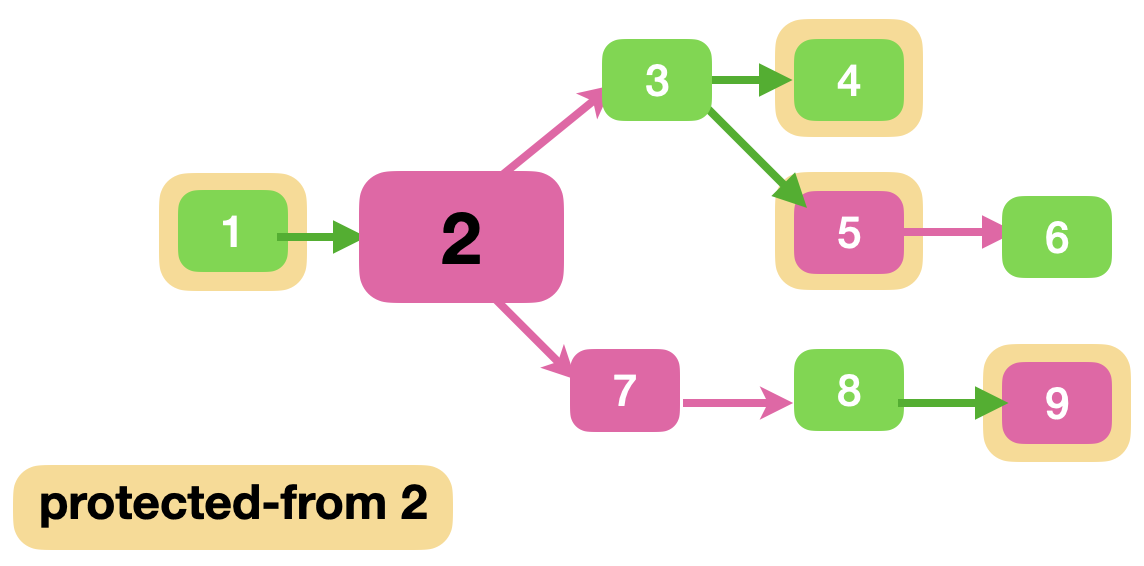
\includegraphics[width=\linewidth]{diagrams/prfC.png}
} 
\\
\hline
protected from $o_5$
&
protected from $o_7$
&
protected from $o_2$
\\
\hline \hline
\end{tabular}
   \caption{Protected From }
   \label{fig:ProtectedFrom}
 \end{figure}
 
 
Figure \ref{fig:ProtectedFrom} illustrates the concept of relative protection. All the pink objects are external, and the green objects are internal. The left pane shows the objects that are protected from $o_5$\footnote{QUESTION: is is $5$ or $o_5$?}, the middle pane shows the objects protected from $o_7$, and the right pane shows the objects protected from $o_2$. We highlight the protected objects in yellow. Thus, all objects except $o_6$ are protected from $o_5$;\ all objects expect $o_8$ are protected from $o_7$;\ and all objects except $o_3$, $o_7$, and $o_8$ are protected from $o_2$. 

Note that $o_8$ is not protected from $o_2$ because there is a path from $o_2$ to $0_8$ which only traverses external objects. Note also, that even though $o_9$ is external, it is protected from $o_7$.
We do not consider protection from the internal objects -- c.f. lemma \ref{lemma:internalProtects}.

\vspace{.1in}

An object is protected, if it is protected from all locally reachable objects.\footnote{TODO: motivate; many external objects, no matter which one has unprotected access to an object }
\begin{definition}[Satisfaction 
of Assertions by module and  state  continued -- Protection] 
\label{def:chainmail-protection}
We continue the definitions in \ref{def:chainmail-semantics}, \ref{def:chainmail-protectionFrom } and  define   
\begin{enumerate}
\item
$\satisfiesA{M}{\sigma} {\inside {\re}}$  \ \ \ iff \ \ \ 
\begin{enumerate}
\item
{$\forall \alpha.[ \  \LRelevant {\alpha}  {\sigma}\ \Longrightarrow \ \  \satisfiesA{M}{\sigma}{\protectedFrom{\re} {{\alpha}}}\ ] $}, \ \ \ and 
\item
$\satisfiesA{M}{\sigma}{\external{\prg{this}}}\ \ \Longrightarrow\ \ \forall x\in dom(\sigma).\satisfiesA{M}{\sigma}{x\neq \re}$
\end{enumerate}
\end{enumerate}
\end{definition}
 
 TODO explain
 
\begin{figure}[htb]
\begin{tabular}{|c|c|c|}
\hline \\
\resizebox{4.5cm}{!}{
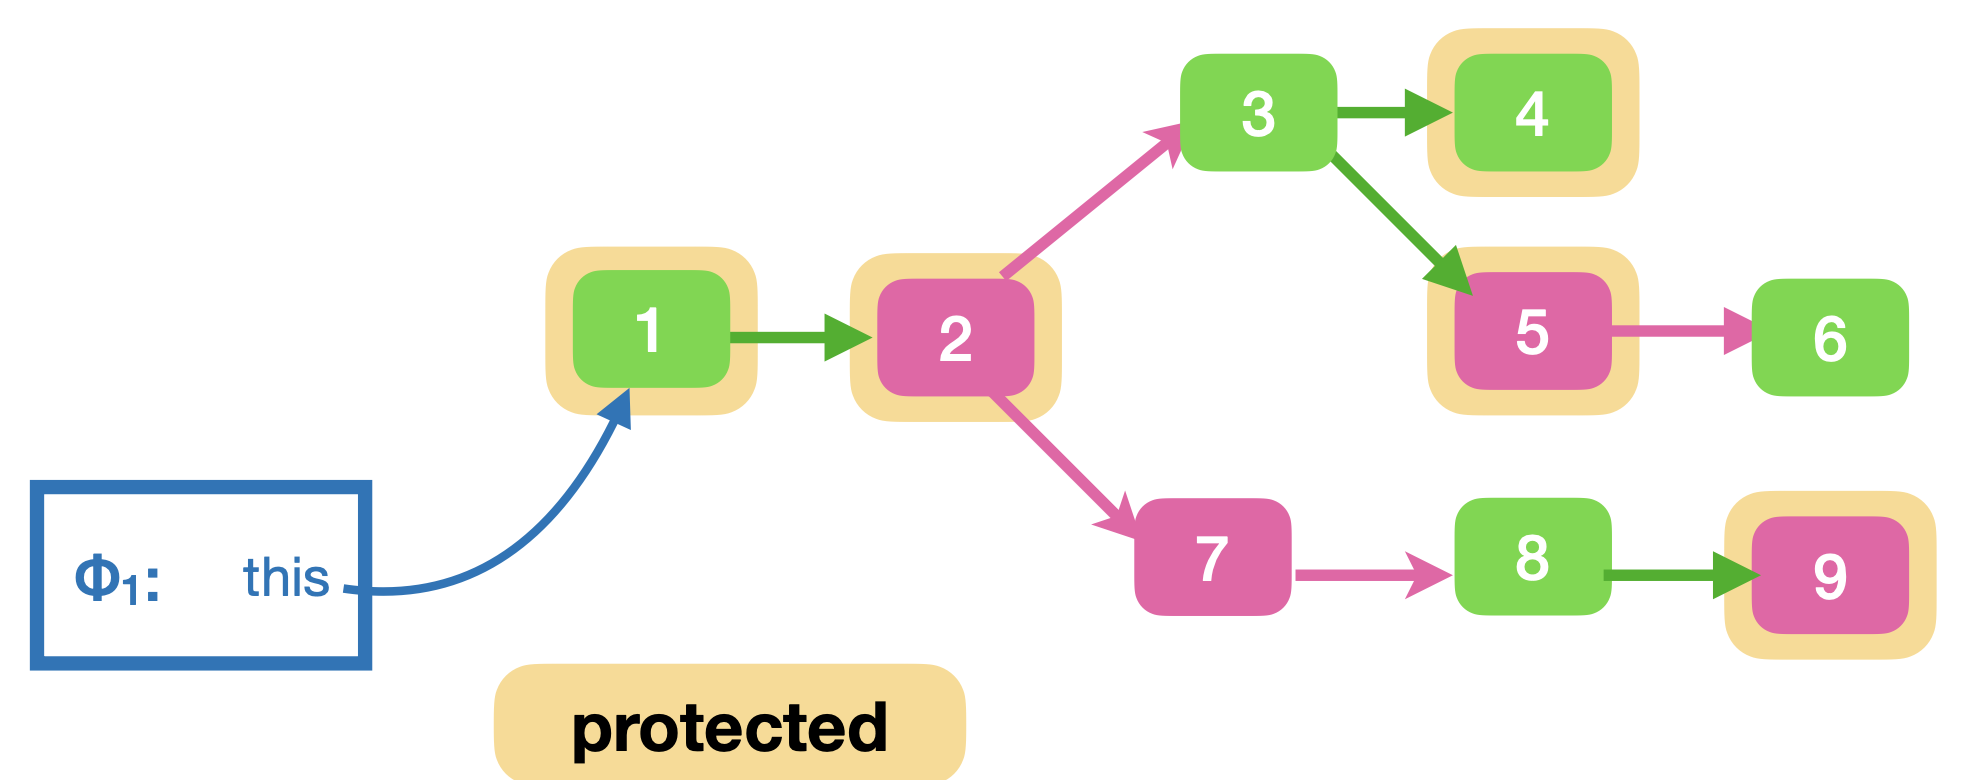
\includegraphics[width=\linewidth]{diagrams/prtFirst.png}
} 
&
\resizebox{4.5cm}{!}{
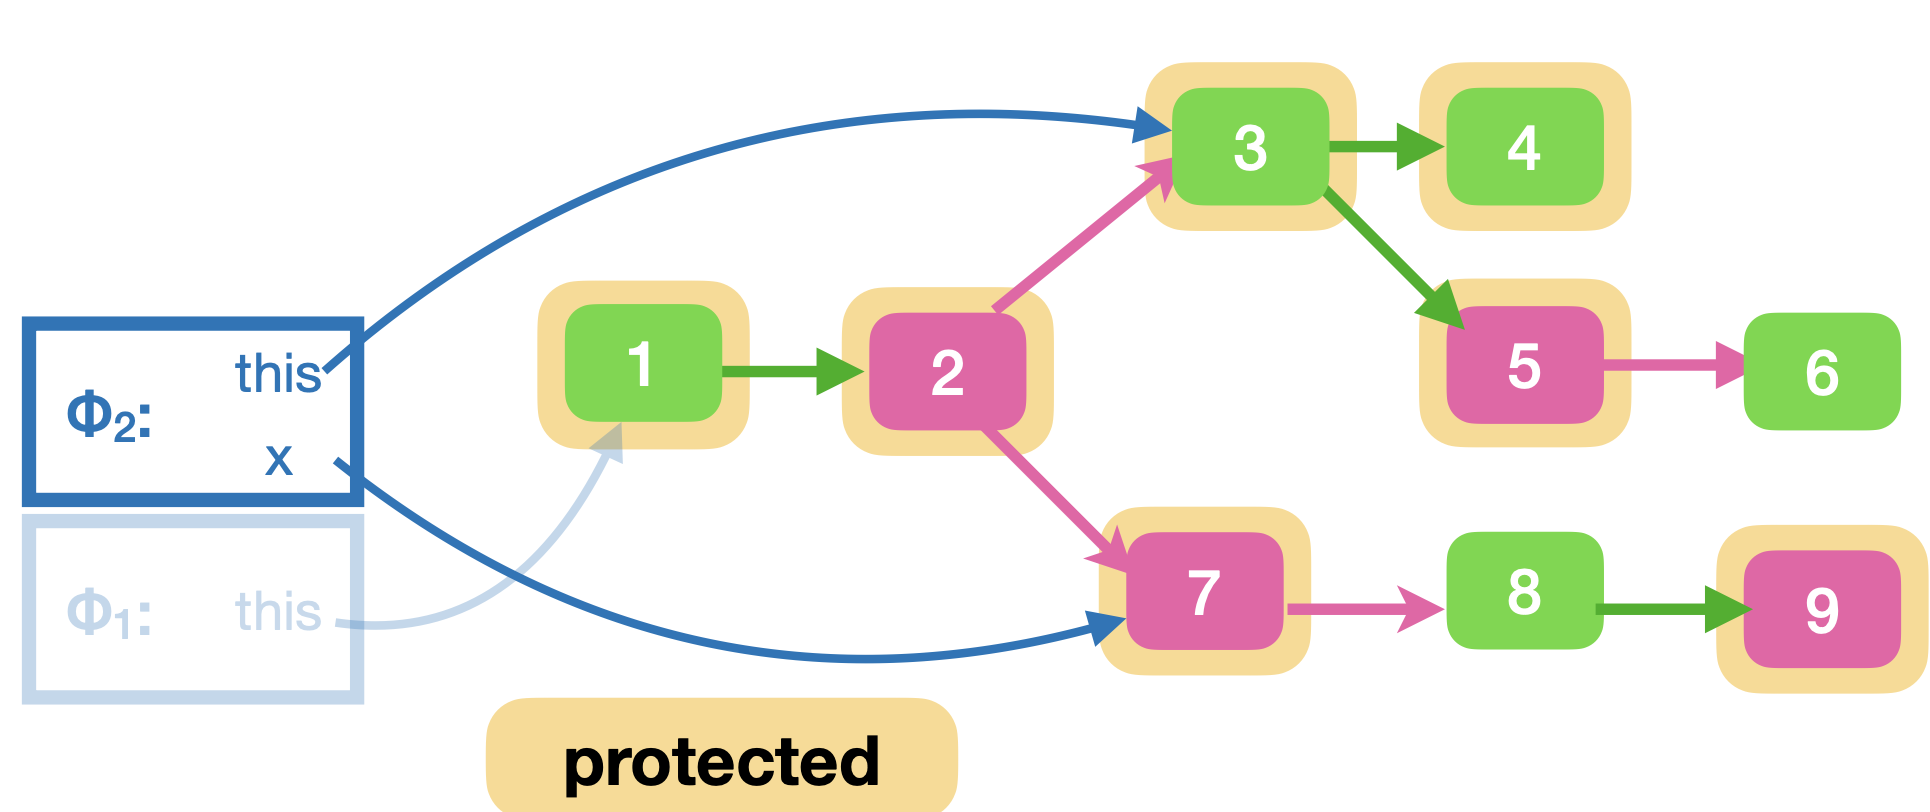
\includegraphics[width=\linewidth]{diagrams/prtSecond.png}
} 
&
\resizebox{4.5cm}{!}{
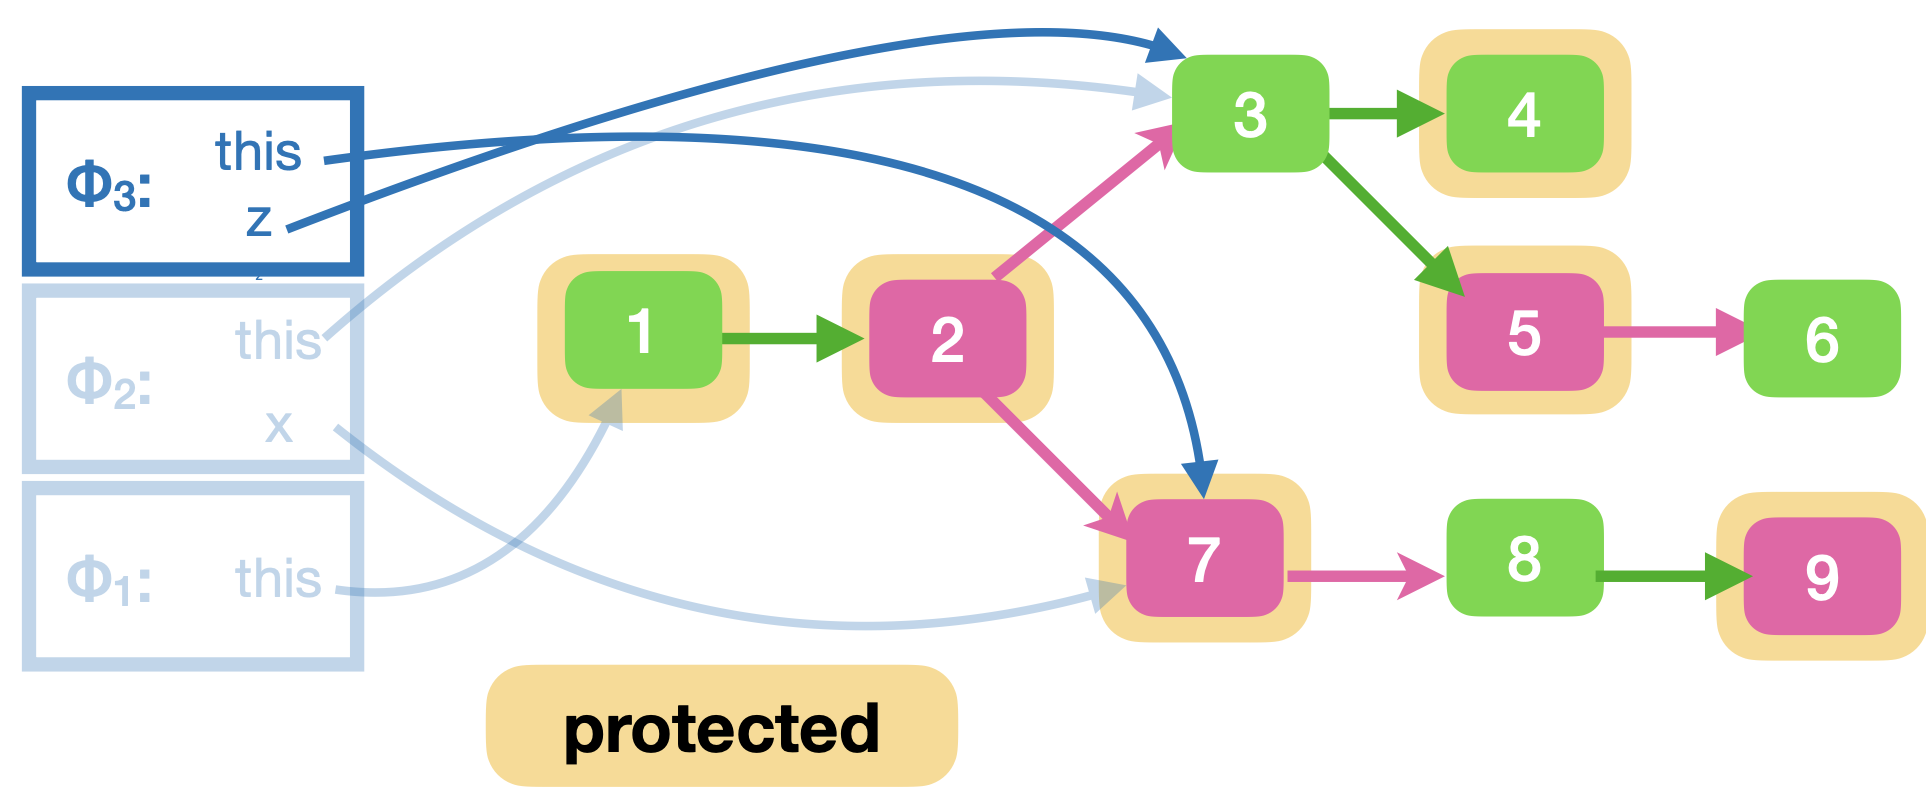
\includegraphics[width=\linewidth]{diagrams/prtLast.png}
} 
\\
\hline
protected  ...
&
protected ...
&
protected  ..
\\
\hline \hline

\end{tabular}
   \caption{Protected \\
 }
   \label{fig:Protected}
 \end{figure}
 
 Figure \ref{fig:Protected} illustrates the concepts  .... The locally reachable objects for the three states are as in Fig \ref{fig:LReachable} ..
 
 \subsection{Discussion of the semantics of assertions}
 
 {Both existential and universal quantification (defined in \ref{quant1} and \ref{quant2}) is done over all objects which are transitively 
accessible any frame in the stack (as in OOPSLA). But note that $\satisfiesA{M}{\sigma} {\inside {y}}$ only considers objects that are locally reachable ..

We do not include quantification over primitive types such as integers as \LangOO is too simple. The 
Coq mechanisation does include primitive types.}
 
\footnote{{. TODO: Do we prove the implications as in TACAS, or just rely on TACAS? -- perhaps the former, since we have some new primitives? hmhh}}



\section{Specifications}

\noindent
The syntax of  \SpecLang specifications is given below
 
\begin{definition}  

\noindent
{\emph{{Syntax of \SpecLang Specifications}}}

\label{f:holistic-syntax}
\[
\begin{syntax}
\syntaxElement{S}{}
		  {\syntaxline
                               {\OneStateQ {\overline {x:C}} {A} }	
				{\TwoStatesQ {\overline {x:C}} {A} {A} }	
				{S\, \wedge \, S}
		 \endsyntaxline
		}
\endSyntaxElement\\
\end{syntax}
\]
\end{definition}

TODO motivate the rest

\subsubsection{Arising States and {Arising} External States}

{TODO: here perhaps more motivation for external?\footnote{Here what we had: As discussed in \S \ref{s:approach}, 
{open world specifications need to be able to provide}
guarantees which hold
during execution of an internal, 
known, trusted module $M$ when linked together with any
unknown, untrusted, module $M_{ext}$. These guarantees need only hold 
when the external module is executing; we are not concerned if they are
temporarily broken by the internal module. Therefore, we are only interested in states where the
executing object (\prg{this}) is an external object. 
To express our focus on external states, we define the  \emph{external states semantics}, of the form 
$\reduction{M_{ext}}{M}{\sigma}{\sigma'}$, where $M_{ext}$ is the external
module, and $M$ is the internal module, and where we
collapse all internal steps into one single step.
}}

{A state $\sigma$ is \emph{arising},}  written $\arising{\sigma}{M}$, {if it  may arise}  % by observable states} 
by execution
starting at some initial configuration:


\begin{definition}[Arising  States]
\label{def:arising}
For modules $M$ and $M_{ext}$ we define arising and arising external states as follows:

\begin{itemize}
\item
 a state $\sigma$ is 
{ an \emph{arising} state, formally \ \ \  $\arising{\sigma}{M}$,\ \ \ 
if and only if there exists some $\sigma_0$ such that $\initial{\sigma_0}$ and
$M, {\sigma_0} \leadsto^* {\sigma}$.}
\item
{A a state $\sigma$ is 
called an \emph{arising} state, formally\ \ \ \  $\extArising{\sigma}{M_{ext}}{M}$,\ \ \ \
if and only if $\arising{\sigma}{M_{ext}*M}$ and $M, \sigma \models \external{\prg{this}}$.}
\end{itemize}
\end{definition}


An \emph{Initial} state's heap contains a single object of class \prg{Object}, and
its  stack   consists of a single frame, whose local variable map is a
mapping from \prg{this} to the single object, and whose continuation is  any statement.
(See Definition %s \ref{def:initial} and 
\ref{def:arising} and the 
{appendices %of the full paper 
\cite{necessityFull}).}



%{
%\begin{definition}[??? Semantics]
%\label{def:up-reduce}
%For    module  $M$  and     states $\sigma$, $\sigma'$, 
%we say that $\ \ \ \ \ \ \ \ \ M {\sigma}\leadstoUp {\sigma'}\ \ \ \ \ \ \ \ $ if and only if there exist 
%$n\in\mathbb{N}$, and states $\sigma_0$,...$\sigma_n$, such that
%\begin{enumerate}
%\item
%\label{up1}
%$\sigma$=$\sigma_1$, and  $\sigma'$=$\sigma_n$,
%\item
%\label{up2}
%$M, \sigma_i \leadsto \sigma_{i+1}$  \ \ \ for all $i\in [{1}..n)$,
%\item
%\label{up3}
%{$| \sigma_1 | \leq | \sigma_i |$ \ \ \  for all $i\in [1..n]$,}
%\end{enumerate} 
%\end{definition}
%}

\begin{figure}[htb]
\begin{tabular}{|c|}
\hline \\
\resizebox{8cm}{!}{
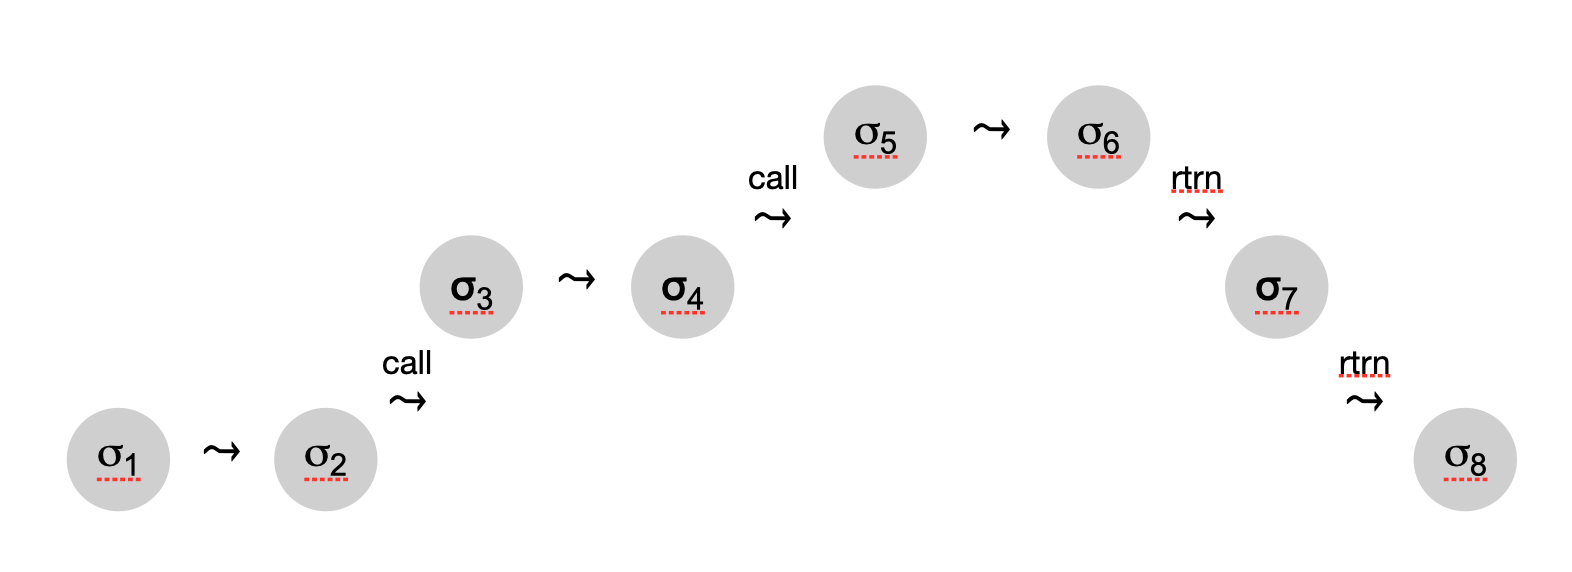
\includegraphics[width=\linewidth]{diagrams/up1.png}
} 
\\
\hline
\\
\begin{tabular}{c|c|c}
%TRAD
$M, {\sigma_3} \leadsto  \sigma_4 $ & 
%REC
  $\leadstoRec  M  {\sigma_3} {\sigma_3}  {\sigma_4} $ & 
  %TERM 
  $\leadstoFin {M} {\sigma_3} {\sigma_7}$
\\
%TRAD
 $M, {\sigma_3} \leadsto^*  \sigma_8 $ & 
%REC
$\neg(\leadstoRecStar M {\sigma_3} {\sigma_3}   {\sigma_8})$ 
&
%REM
\leadstoFin {M} {\sigma_4} {\sigma_7} \\
%TRAD
&
%REC
 \leadstoRecStar M {\sigma_3} {\sigma_1}   {\sigma_8}
  &
   \\
 \hline
 \\
 $\leadsto$
 &
 $\leadsto_{\sigma}$
 &
  $\leadstoFin {\_} {\_} {\_}$
\\
\hline
\end{tabular}
\end{tabular}
   \caption{Illustrating  % $\leadsto$ and  $\leadsto_{\sigma}$  and Semantics; Illustration $\leadstoFin {\_} {\_} {\_}$ 
   deep, shall, and terminating semantics
     (Def. \ref{def:deep}, and \ref{def:shallow:term})%
    }
   \label{fig:UpSemantics}
 \end{figure}

 
{ The $\leadsto_{\sigma}$ relation is transitive, in the sense that $\leadstoRecStar {M}  {\sigma_1} {\sigma'} {\sigma_2}$ and $\leadstoRecStar  {M}  {\sigma_2} {\sigma'} {\sigma_3}$ implies that $\leadstoRecStar {M}  {\sigma_1} {\sigma'} {\sigma_3}$.}
 
 




 




\subsubsection{ Semantics of \SpecLang Specifications}
We now  define what it means for  a module  $M$ to satisfy specification  $S$, written as $M \vDash S$. The
 
\begin{definition}% [Semantics of \SpecLang Specifications]

We define $\satisfies{M}{{S}}$ by cases over the three possible syntactic forms.
For any assertions   $A_1$, $A_2$, and $A$: \\

\label{def:necessity-semantics}

\begin{tabular}{l l c l }

$\bullet$ & $\satisfies{M}{\OneStateQ {\overline {x:C}} {A} 	}$& iff & 
for all $M_{ext}$, $\sigma$, $\overline{x}$, such that $\overline{x}$  are free in $\sigma$, \\
  & & & $ \extArising{\sigma}{M_{ext}}{M}$ % \ \wedge 
$ \ \Longrightarrow \  $  % \\ & & &  $ \satisfiesA{M}{\sigma[\overline{x\mapsto o}]}{A} $
{$ \satisfiesA{M}{\sigma}{\forall \overline{x:C}.A}$}\footnote{{This means that we require all objects to satisfy even if not locally relevant}}
\\
\\
$\bullet$ & $\satisfies{M}{\TwoStatesQ {\overline {x:C}} {A}{A'}}$& iff & 
for all $M_{ext}$, $\sigma$, $\overline{x}$, $\overline{o}$ such that $\overline{x}$  are free in $\sigma$  \\
& & &
${\extArising{\sigma}{M_{ext}}{M}} \ \wedge\  \GRelevant {\overline o}  \sigma \wedge \ $\footnote{{notice that we are asking for globally relevant objects}}\\
& & & $ \satisfiesA{M}{\sigma[\overline{x\mapsto o}]}{\overline {x:C}}  \ \ \wedge\ \  \satisfiesA{M}{\sigma[\overline{x\mapsto o}]}{A} \ \ \wedge$ \\ 
& & &
$\red{\leadstoRecStar {M_{ext}\!\circ \!M}{\sigma}{\sigma} {\sigma'} } \ \ \wedge\ \  M, \sigma' \models {\external{\prg{this}}}$ \\
& & & $ \Longrightarrow $ \\
& & & $ \satisfiesA{M}{\sigma'[\overline{x\mapsto o}]}{A'} $
\\
\\
$\bullet$ &  $\satisfies{M}{S\, \wedge\, S'}$ &   iff   & $\satisfies{M}{S}\ \wedge \ \satisfies{M}{S'}$
\end{tabular} 

 
\end{definition} 


  
  \footnote{{TODO: Make an example that demonstrates the difference if in the second bullet we had asked for locally relevant objects ${\overline o}$.}}
 
\footnote{{TODO Notice that we assume that $\overline x$ are not free in $A$ -- cf Barendregt convention.}}

\footnote{TODO: explain why we did not require the stronger $\leadstoFin{M_{ext}\!\circ \!M}{\sigma}{\sigma'}$ rather than $\leadstoRecStar {M_{ext}\!\circ \!M}{\sigma}{\sigma} {\sigma'}$.}
% Note that the requirements that $\extArising{\sigma}{M_{ext}}{M}$ and $\leadstoFin{M_{ext}\circ M}{\sigma}{\sigma'} $ imply that
% $M, \sigma' \models {\external{\prg{this}}}$



{We demonstrate the meaning of ${\TwoStatesQ {\overline {x:C}} {A}{A'}}$ in Fig. where we assume that the pink states (\ie   ${\sigma_1}$, 
 ${\sigma_2}$,  ${\sigma_3}$,  ${\sigma_6}$,  ${\sigma_8}$ are external, and the green states (\ie   ${\sigma_3}$, 
 ${\sigma_4}$,  and ${\sigma_7}$ are internal.}
 
 \begin{figure}[htb]
\begin{tabular}{|c|}
\hline \\
\resizebox{8cm}{!}{
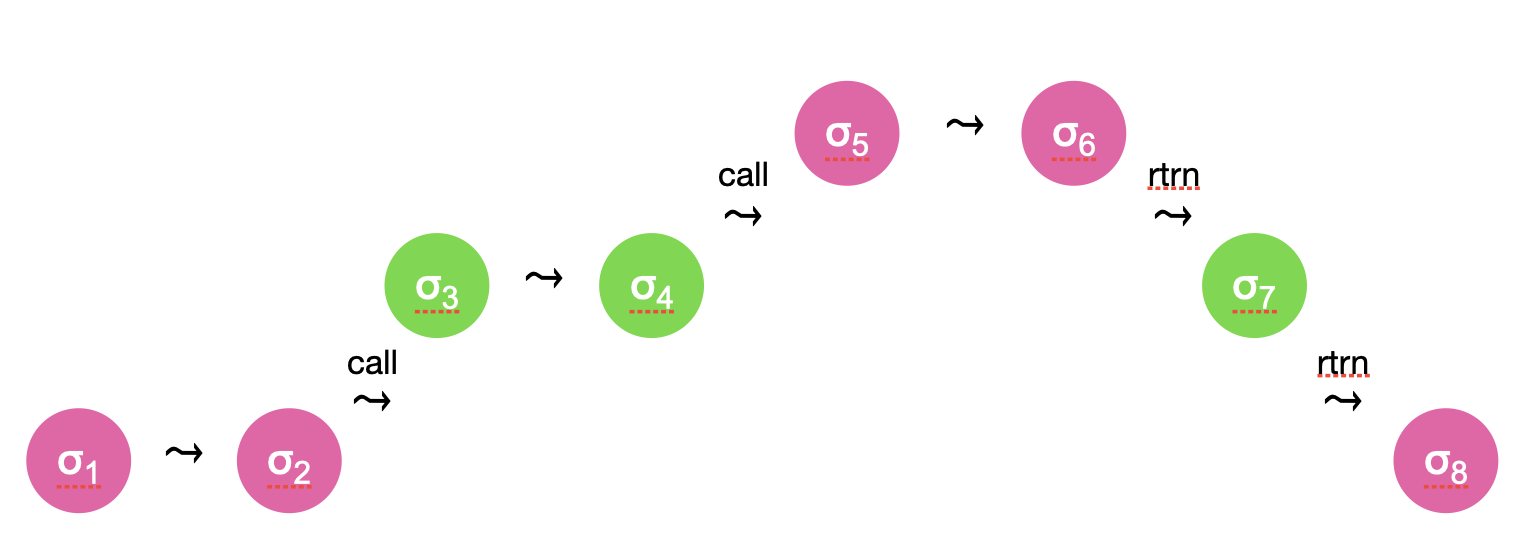
\includegraphics[width=\linewidth]{diagrams/SemFutSpec.png}, 
} 
\\
\hline
\\
\begin{tabular}{lclclcl} 
$ {\sigma_1} \leadsto  \sigma_2 $ preserves $A_0$ & &
$ {\sigma_2} \leadsto^*  \sigma_6 $ preserves $A_0$ \\
$ {\sigma_1} \leadsto  \sigma_8 $ preserves $A_0$ & &
$ {\sigma_5} \leadsto^* \sigma_8 $ does not preserve $A_0$\\
$ {\sigma_3} \leadsto  \sigma_4 $ does not preserve $A_0$ & &
$ {\sigma_2} \leadsto  \sigma_7 $ does not preserve $A_0$
\\
\hline
\end{tabular}
\end{tabular}
   \caption{Illustrating  the meaning on ${\TwoStatesQ {\overline {x:C}} {A_0}{A_0}}$    }
   \label{fig:TwoStateSemantics}
 \end{figure}
 
\subsection{Specification Examples}
\noindent
As an example, consider the following    specifications:

\begin{tabular}{lcll}
$S_1$   &     $\triangleq$   & $\OneStateQ{\prg{a}:\prg{Account} } {\inside{\prg{a}}} $
 \\
 $S_2$   &     $\triangleq$   & $\OneStateQ{\prg{a}:\prg{Account} } {\inside{\prg{a.password}}} $
 \\
 $S_3$   & $\triangleq$   &  $\TwoStatesQ {\prg{a}:\prg{Account}}  {\inside{\prg{a}}} {\inside{\prg{a}}} $
 \\
 $S_4$   & $\triangleq$   &  $\TwoStatesQ {\prg{a}:\prg{Account}}  {\inside{\prg{a.password}}} {\inside{\prg{a.password}}}$
 \\
$S_5$ & $\triangleq$   &
 $\forall \prg{a}:\prg{Account}.\forall \prg{b}:\prg{int}.$\\
  &  &  $\FirstState{\inside{\prg{a}} \wedge \prg{a.balance}=\prg{b}} 
\  \SecondState{ \prg{a.balance}= \prg{b} }$
\\
$S_6$ & $\triangleq$   &
  $\forall \prg{a}:\prg{Account}.\forall \prg{b}:\prg{int}.$\\
  &  &  $\FirstState{\inside{\prg{a.password}} \wedge \prg{a.balance}=\prg{b}} 
\  \SecondState{ \prg{a.balance}\geq \prg{b} }$
 \end{tabular}

\vspace{.2cm}
Now consider our modules from earlier. We have that

\begin{tabular}{lllllll}
$\ModA \not\models S_1$  & & $\ModA \not\models S_2$ &&  $\ModB \not\models S_1$ &  &$\ModB \not\models S_2$ \\
$\ModA \models S_3$ & &   $\ModA \models S_4$ & &  $\ModB  \models S_3$ & &  $\ModB  \not\models S_4$ \\
$\ModA \models S_5$ & &  $\ModA \models S_6$ & & $\ModB  \models S_5$ & & $\ModB   \not\models S_6$ \\
\end{tabular}

\vspace{.6cm}
Consider also  $S_{4a}$ which is a variation of $S_4$, as well as $S_7$, which ...

\begin{tabular}{lcll}
$S_{4a}$   &     $\triangleq$   &   ${\TwoStatesQ {\prg{a}:\prg{Account}.\prg{p}:\prg{Password}}  {\prg{p}=\prg{a.password} \wedge \inside{\prg{p}}}{\inside{\prg{p}}} }$
 \\
$S_7$ & $\triangleq$   & ${\TwoStatesQ {\prg{a}:\prg{Account}.\prg{p}:\prg{Password}}  {\prg{p}=\prg{a.password}} {\prg{p}=\prg{a.password}} }$
 \end{tabular}
 
 \noindent
 Fort these specifications
 
 \begin{tabular}{lllllll}
$\ModA  \models S_7$  & & $\ModB \not\models S_7$ &&  $\ModC \not\models S_7$ \\
\end{tabular}

\subsection{Tautological assertions, and Specification Implication}

\begin{definition}[Satisfaction of Assertions by a module] 
\label{def:assertion-inference-semantics}
We define satisfaction of an assertion $A$ by a  module $M$ as:
\begin{itemize}
\item
$M \vDash A$   \ \ \ iff \ \ \  $\forall M_{ext}. \forall \sigma.[\ \extArising{\sigma}{M_{ext}}{M} \ \Longrightarrow \ \ \satisfiesA{M}{\sigma}{e}\ \ ]$
\end{itemize}
\end{definition}

TODO: Here we will say that assertions are classical, as proven in FASE

\begin{definition}[Stronger Specifications] 
\label{def:specification-implication-semantics}
We define when a specification $S$ is stronger than another specification $S'$  in the context of a  module: 
 \begin{itemize}[itemsep=5pt]
\item 
$\stronger M  S  {S'}$   \ \ \ iff \ \ \  $M\models S$ implies $M \models S'$
\item
$\strongerEq M  S  {S'}$   \ \ \ iff \ \ \ $\stronger M  S  {S'}$  \ and \  $\stronger M   {S'} S$    
\end{itemize}
\end{definition}

We know about stronger specifications:

\begin{lemma}
Consider assertions $A$, $A'$, variable $y$ free in $A$, specifications $S$, $S'$, and module $M$:
\begin{itemize} [topsep=6pt,itemsep=5pt,parsep=0pt,partopsep=0pt]
\item
$\stronger M {\OneStateQ {\overline {x:C}}  {A}}  {\TwoStatesQ {\overline {x:C}} {A}{A}} $ 
    \item
 $\strongerEq  M  {\OneStateQ    {y:\prg{Object}}   {\forall \overline {x:C}[ A ] } } 
    {\OneStateQ {\overline {x:C}}  {A}} $.
\item
$  M  \models (  \overline {x:C} \wedge A) \rightarrow A'$ \ \ \  implies \ \  \ $\stronger M  {\OneStateQ {\overline {x:C}} {A}}    {\OneStateQ {\overline {x:C}} {A'}}$
\item
  \ $\stronger M  { \TwoStatesQ {y:\prg{Object}}  {\forall x:C.[A]} {\forall x:C.[A']} }    {\TwoStatesQ {\overline {x:C}} {A}{A'}} $

\item
$\stronger M  S {S''}$ and $\stronger M {S''} {S'}$\ \  implies \ \ $\stronger M S  {S'}$.
\end{itemize}

\end{lemma}



